% !TEX root = SCPROG.tex
% This work is licensed under the Creative Commons
% Attribution-NonCommercial-ShareAlike 4.0 International License. To view a copy
% of this license, visit http://creativecommons.org/licenses/by-nc-sa/4.0/ or
% send a letter to Creative Commons, PO Box 1866, Mountain View, CA 94042, USA.

\chapter{Die Java-Welt}
\section{Was ist Java? Java-Komponenten und -Tools}

Java besteht aus dem \define{Java Runtime Environment (JRE)} und dem \define{Java Development Kit (JDK)}.
Das JRE braucht man, um Java (bzw. den erzeugten Bytecode) auszuführen.
das JRE besteht wiederum aus aus der \define{Java Virtual Machine (JVM)} und der \define{Java Class Library (JCL)}.
Das JDK benötigt man um Java-Programme zu kompilieren.
Es besteht aus:
\index{Java Development Kit}\index{JDK|see{Java Development Kit}}
\index{Java Runtime Environment}\index{JRE|see{Java Runtime Environment}}\index{Java Virtual Machine}\index{JVM|see{Java Virtual Machine}}
\index{Java Class Library}\index{JCL|see{Java Class Library}}
\begin{itemize}
	\item javac (Java Compiler)
	\item javadoc (Java Documentation); Javadoc-Kommentar: \code{/**$\ldots$*/}
	\item loader
	\item applet viewer
	\item jdb (Java Debugger)
	\item jar (Java Archive)
\end{itemize}

Früher hat man \define{graphical user interface (GUI)} mit dem \define{Abstract Windowing Toolkit (AWT)} in Java erstellt.
Es wurde von \define{Swing} abgelöst.
Eine Neuentwicklung auf diesem Gebiet ist \define{JavaFX}, allerdings hat Oracle die Entwicklung von JavaFX schon wieder eingestellt.

\section{Historisches, Java-Versionen}

\begin{itemize}
	\item 1991: Java hieß noch \define{oak}: James Gosling ist der "Vater von Java" (Sun Microsystems)
	\item 1995: Oak wurde Java umbenannt; Java war im ersten Browser (\undefine{Netscape}) eingebettet
	\item 1996: JDK 1.0: erster just-in-time (JIT) compiler
	\item 1999: Java 2 Platform = Java 1.2
	\item 2002: J2SE = Java 1.4 (SE = Standard Edition)
	\item 2004/05: J2SE 5[.0]  = Java 5: generics, enums, varargs, automatic boxing/unboxing (primitive type $\leftrightarrow$ wrapper type)
	\item 2006/07: Java SE 6 = Java 6
	\item 2007: große Teile des Java Systems wurden übergeben an \undefine{OpenJDK} (open source)
	\item 27.01.2010: Orcale übernimmt Sun Microsystems: Java, MySQL, XML, JRuby, Solaris, OpenOffice wurde Teil von LibreOffice
	\item 2011: Java 7
	\item 2014: Java 8: $\lambda$-expressions (=: closures) $\leadsto$ funktionale Programmierung; JavaFX wurde eingeführt und sollte Swing ersetzen
	\item Sep. 2017: Java 9: ahead-of-time compilation
	\item Ma. 2018: Java 10: neuer JIT compiler, neuer Garbage Colletor (GC)
	\item Sep. 2018: Java 11: entfernt wurden: JavaFX, Jave EE (Enterprise Edition), Corba
	\item Mar. 2019: Java 12
\end{itemize}

\section{Prinzipien des objektorientierten Programmierens (OOPs)}
\begin{enumerate}[label=(\arabic*)]\index{Modularisierung}\index{Vererbung}\index{Polymorphie}\index{dynamisches Binden}\index{spätes Binden}
	\item \ul{Modularisierung (Module / Klassen)} $\leftrightsquigarrow$ abstrakte Datentypen (ADT)\\
	Datenkapselung: Objekte haben Daten und Methoden
	\item \ul{Vererbung:} Beziehung / Hierarchie zwischen Klassen\\
	in Java: nur Einfachvererbung (d.h. jede Klasse hat genau eine Superklasse / Mutterklasse, außer \code{object})\\
	$\implies$ Klassenhierarchie ist ein Baum
	\item \ul{Polymorphie:}
	\begin{itemize}
		\item \ul{von Variablen:} eine Variable vom Type $T$ kann ein Objekt von jeden (direkten oder indirekten) Subtyp von $X$ enthalten / referenzieren.\\
		Schreibe $S\subseteq T$ oder $S\subset T$ für Subtypen
		\item \ul{von Methoden:} führt zu \ref{item:OOP(4)}
	\end{itemize}
	\item \ul{Dynamisches / spätes Binden:}\label{item:OOP(4)}
	Es wird zur Laufzeit entschieden, welche Methode aufgerufen wird.
\end{enumerate}

Außerdem gehört noch zu OOP: dynamische Speicherverwaltung, Referenzvariablen, Überladung / Überschreibung von Methoden, Exception Handling, generische Datentyen, $\ldots$

\begin{figure}[H] % oder ht!
	\begin{center}
		% A simple Tree
% Author: Stefan Kottwitz
% https://www.packtpub.com/hardware-and-creative/latex-cookbook

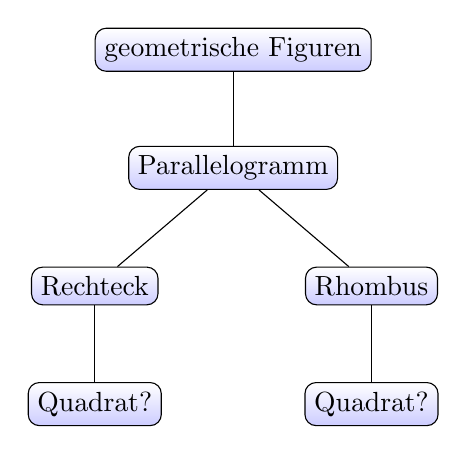
\begin{tikzpicture}[sibling distance=10em,
  every node/.style = {shape=rectangle, rounded corners,
    draw, align=center,
    top color=white, bottom color=blue!20}]]
  \node {geometrische Figuren}
    child { node {Parallelogramm} 
      child { node {Rechteck} 
      	child { node {Quadrat?}}}
      child { node {Rhombus} 
        child { node {Quadrat?} }}};
\end{tikzpicture}
		\caption{Einfachvererbung: Ist ein Quadrat ein Rechteck oder ein Rhomus?}
		\label{Abb:einfachvererbung}
	\end{center}
\end{figure}

\section{Anwendungsgebiete, Einschränkungen, Vor- und Nachteile}

